\begin{table}
    \centering
    \begin{center}
        \begin{tabular}{l c c c c c c}
        \toprule
        Setting & \shortstack{LAMBADA\\(acc)} & \shortstack{LAMBADA\\(ppl)} & \shortstack{StoryCloze\\(acc)} & \shortstack{HellaSwag\\(acc)}\\ 
        \midrule
        SOTA & 68.0\textsuperscript{\textit{a}} & 8.63\textsuperscript{\textit{b}}  & \textbf{91.8}\textsuperscript{\textit{c}} & \textbf{85.6}\textsuperscript{\textit{d}}\\ 
        GPT-3 Zero-Shot & \textbf{76.2} & \textbf{3.00}   & 83.2 & 78.9\\
        GPT-3 One-Shot & \textbf{72.5} &\textbf{3.35} &  84.7 & 78.1\\
        GPT-3 Few-Shot & \textbf{86.4} & \textbf{1.92} & 87.7 & 79.3\\
        \bottomrule
        \end{tabular}
    \end{center}
    \caption{\textbf{Performance on cloze and completion tasks.} GPT-3 significantly improves SOTA on LAMBADA while achieving respectable performance on two difficult completion prediction datasets. \textsuperscript{\textit{a}}\cite{turing_17m} \textsuperscript{\textit{b}}\cite{radford2019language} \textsuperscript{\textit{c}}\cite{li2019story} \textsuperscript{\textit{d}}\cite{liu2020alum} }
    \label{table:completion}
\end{table}
\begin{figure}
\vspace{-1em}\centering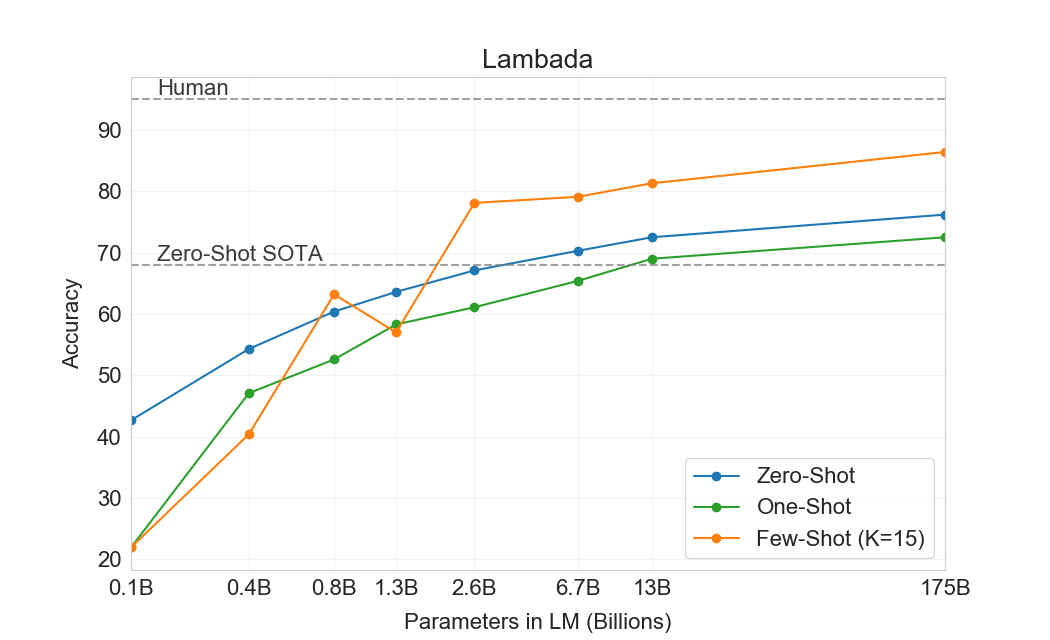
\includegraphics[width=0.8\linewidth]{graphs/scale_plots/lambada_acc_test.png}
\caption{On LAMBADA, the few-shot capability of language models results in a strong boost to accuracy. GPT-3 2.7B outperforms the SOTA 17B parameter Turing-NLG \cite{turing_17m} in this setting, and GPT-3 175B advances the state of the art by 18\%.  Note zero-shot uses a different format from one-shot and few-shot as described in the text.}
\label{graph:lambada}
\end{figure}


The LAMBADA dataset \cite{paperno2016lambada} tests the modeling of long-range dependencies in text -- the model is asked to predict the last word of sentences which require reading a paragraph of context. It has recently been suggested that the continued scaling of language models is yielding diminishing returns on this difficult benchmark. \cite{bisk2020experience} reflect on the small 1.5\% improvement achieved by a doubling of model size between two recent state of the art results (\cite{shoeybi2019megatronlm} and \cite{turing_17m}) and argue that ``continuing to expand hardware and data sizes by orders of magnitude is not the path forward''. We find that path is still promising and in a zero-shot setting GPT-3 achieves 76\% on LAMBADA, a gain of 8\% over the previous state of the art.

LAMBADA is also a demonstration of the flexibility of few-shot learning as it provides a way to address a problem that classically occurs with this dataset. Although the completion in LAMBADA is always the last word in a sentence, a standard language model has no way of knowing this detail. It thus assigns probability not only to the correct ending but also to other valid continuations of the paragraph. This problem has been partially addressed in the past with stop-word filters \cite{radford2019language} (which ban ``continuation'' words). The few-shot setting instead allows us to ``frame'' the task as a cloze-test and allows the language model to infer from examples that a completion of exactly one word is desired. We use the following fill-in-the-blank format:

\hspace{3cm}Alice was friends with Bob.  Alice went to visit her friend \underline{\hspace{1cm}}. $\to$ Bob

\hspace{3cm}George bought some baseball equipment, a ball, a glove, and a \underline{\hspace{1cm}}. $\to$ 

When presented with examples formatted this way, GPT-3 achieves 86.4\% accuracy in the few-shot setting, an increase of over 18\% from the previous state-of-the-art. We observe that few-shot performance improves strongly with model size. While this setting decreases the performance of the smallest model by almost 20\%, for GPT-3 it improves accuracy by 10\%. Finally, the fill-in-blank method is not effective one-shot, where it always performs worse than the zero-shot setting. Perhaps this is because all models still require several examples to recognize the pattern.

One note of caution is that an analysis of test set contamination identified that a significant minority of the LAMBADA dataset appears to be present in our training data -- however analysis performed in Section \ref{section:measuring_and_preventing_memorization_of_benchmarks} suggests negligible impact on performance.